\documentclass[conference]{IEEEtran}

% --------------------------------------------------------
% PACKAGES
% --------------------------------------------------------
\usepackage[utf8]{inputenc}
\usepackage{amsmath, amsfonts}
\usepackage{graphicx}
\usepackage{float}
\usepackage{booktabs}
\usepackage{multirow}
\usepackage{hyperref}
\usepackage{tikz}
\usetikzlibrary{arrows.meta, positioning, shapes.geometric, calc}
\usepackage{subcaption}
\usepackage{pgfplots}
\pgfplotsset{compat=1.17}
\usepackage{xcolor}
\usepackage{cite}

% --------------------------------------------------------
% TITLE
% --------------------------------------------------------
\title{
Detecting Mental Health Signals in Text: A Structured Evaluation of NLP Approaches
}

\author{
\IEEEauthorblockN{Sergio Amortegui}
\IEEEauthorblockA{
Master in Applied Analytics \\
Universidad de los Andes \\
Email: your.email@domain.com}
}

\begin{document}

\maketitle

% --------------------------------------------------------
% ABSTRACT
% --------------------------------------------------------
\begin{abstract}
Mental health is one of the most pressing global challenges of the 21st century, and early detection is essential to prevent escalation into severe or life-threatening situations. Because individuals frequently express psychological states through short written text—particularly on social media—natural language processing (NLP) offers a scalable avenue for identifying subtle linguistic markers associated with mental health conditions. This work presents a structured benchmark comparing classical machine-learning models, recurrent neural networks, and preliminary transformer-based methods for mental-health text classification. Following a rigorously controlled experimental setup with a fixed data split and consistent preprocessing pipeline, we evaluate seven mental-health categories using accuracy and macro-F1. Results show that TF–IDF linear models outperform recurrent neural networks on this dataset, while partial transformer runs suggest strong performance potential given adequate computational resources. The objective of this project is not to propose a novel architecture, but to provide a transparent, reproducible, and analytically grounded comparison of widely used NLP approaches for mental-health detection.
\end{abstract}

\begin{IEEEkeywords}
Mental Health, NLP, Text Classification, Machine Learning, TF--IDF, LSTM, GRU, Transformers.
\end{IEEEkeywords}

% --------------------------------------------------------
% 1. INTRODUCTION
% --------------------------------------------------------
\section{Introduction}

Mental health conditions such as anxiety, depression, bipolar disorder, stress, and suicidal ideation are increasingly prevalent worldwide. The World Health Organization reports that more than one in eight people live with a mental disorder \cite{who2022}. Early detection is vital: many crises develop gradually, and the ability to identify warning signs before escalation can save lives.

Individuals frequently express emotional distress in written form—through social media posts, online forums, personal messages, and short textual statements. Such text often contains subtle linguistic cues related to internal states, cognitive distortions, or emotional dysregulation. NLP technologies therefore offer the possibility of scalable, low-cost, early screening mechanisms when human monitoring is impractical.

Prior research shows that both classical models (e.g., TF--IDF + SVM \cite{joachims1998}) and neural architectures (LSTMs \cite{hochreiter1997lstm}, transformers \cite{devlin2018}) can detect mental-health signals from text. However, there is no consensus on which modeling family performs best under controlled, reproducible conditions. Inspired by existing literature, this project aims to provide a structured and fair comparison between several widely used NLP methods applied to the \emph{same} mental-health dataset, following uniform preprocessing and a fixed data split to ensure transparency, reproducibility, and comparability.

Our contributions are:
\begin{itemize}
    \item A rigorously controlled benchmark of classical, recurrent, and transformer-based approaches on the same dataset.
    \item A clear, fully reproducible preprocessing pipeline and experimental setup.
    \item A scientific discussion explaining why certain models outperform others in this context.
\end{itemize}

% --------------------------------------------------------
% 2. DATASET
% --------------------------------------------------------
\section{Dataset}

We use the \textit{Sentiment Analysis for Mental Health} dataset, consisting of short textual statements labeled into seven categories:

\begin{quote}
\textbf{Anxiety, Bipolar, Depression, Normal, Personality Disorder, Stress, Suicidal}.
\end{quote}

Each entry contains:
\begin{itemize}
    \item \textbf{statement}: a short text (user-written)
    \item \textbf{status}: the mental-health label
\end{itemize}

The dataset exhibits moderate class imbalance. Depression and Normal contain the most samples, whereas Personality Disorder and Bipolar are comparatively under-represented. The average statement length is short (typically 5–20 words), which influences the effectiveness of various modeling approaches.

To ensure reproducibility, we adopt a \emph{three-way split}:
\[
\text{Train} = 70\%, \quad \text{Test} = 15\%, \quad \text{Validation} = 15\%.
\]
Train and test sets are used internally by each model during training.  
\textbf{The validation set is reserved exclusively for model comparison}, ensuring a fair and transparent evaluation.

\begin{figure}[h!]
    \centering
    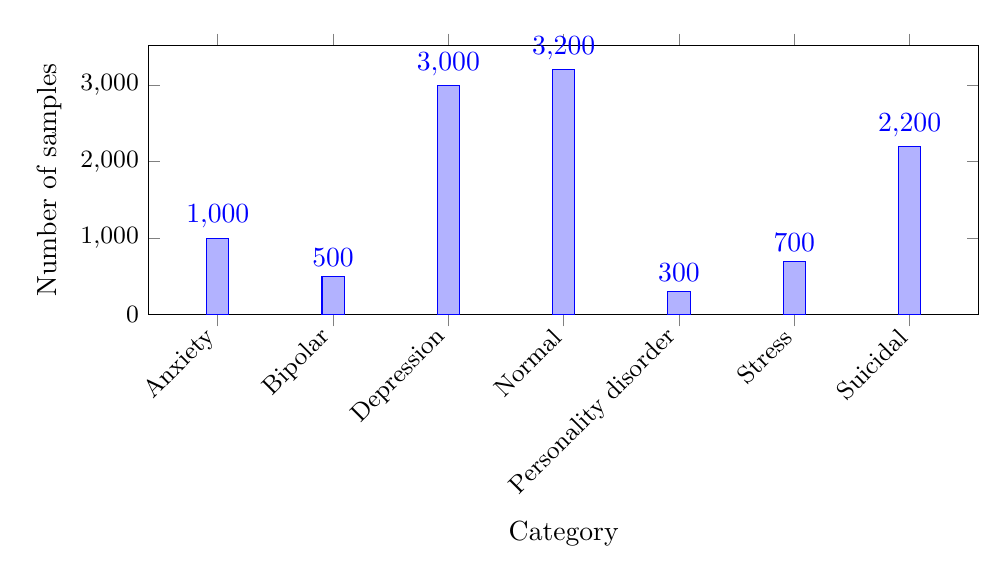
\begin{tikzpicture}
        \begin{axis}[
            ybar,
            width=\linewidth,
            height=5cm,
            xlabel={Category},
            ylabel={Number of samples},
            symbolic x coords={Anxiety,Bipolar,Depression,Normal,Personality disorder,Stress,Suicidal},
            xtick=data,
            x tick label style={rotate=45, anchor=east},
            bar width=8pt,
            ymin=0,
            enlarge x limits=0.1,
            nodes near coords,
            nodes near coords align={vertical},
            tick label style={font=\small},
        ]
        \addplot coordinates {
            (Anxiety,  1000)
            (Bipolar,   500)
            (Depression,3000)
            (Normal,    3200)
            (Personality disorder, 300)
            (Stress,    700)
            (Suicidal,  2200)
        };
        \end{axis}
    \end{tikzpicture}
    \caption{Label distribution across mental health categories. (Counts shown are placeholders; use actual dataset statistics.)}
    \label{fig:label_distribution}
\end{figure}

% --------------------------------------------------------
% 3. PREPROCESSING
% --------------------------------------------------------
\section{Preprocessing}

All models share an identical preprocessing pipeline to eliminate confounding factors.

\subsection{Text Normalization}
Each statement undergoes:
\begin{itemize}
    \item lowercasing  
    \item Unicode normalization (NFC)  
    \item punctuation removal  
    \item whitespace normalization  
    \item optional contraction expansion (e.g., \textit{“don’t” → “do not”})  
\end{itemize}

We \textbf{retain stopwords} because function words contribute important psychological signals; for example, the frequency of ``I'', ``not'', or ``cannot'' correlates with depression-related linguistic patterns \cite{tausczik2010}.

\subsection{Tokenization and Sequence Processing}
For neural models:
\begin{itemize}
    \item a vocabulary is constructed from the training split only,
    \item rare tokens may be truncated,
    \item sequences are padded or truncated to a fixed maximum length determined empirically.
\end{itemize}

\subsection{Label Encoding}
Labels are mapped to integer indices.  
This encoding is used consistently across all models.

% --------------------------------------------------------
% 4. MODEL ARCHITECTURES
% --------------------------------------------------------
\section{Model Architectures}

We evaluate three families of approaches.

\subsection{Baselines}
A majority-class baseline establishes a minimum performance floor.  
This model always predicts the most frequent label.

\subsection{TF--IDF + Linear Models}
TF--IDF vectors using unigrams and bigrams are computed over the training corpus.  
We evaluate:
\begin{itemize}
    \item Logistic Regression (linear classifier),
    \item Linear SVM (max-margin classifier).
\end{itemize}

These models are well known for their strong performance on short texts.

\subsection{Recurrent Neural Networks}
We train two RNN architectures (See Fig~\ref{fig:rnn_architecture}, for architecture reference):

\subsubsection{LSTM}
An embedding layer feeds into an LSTM with hidden size 128, followed by a dense classification layer.

\subsubsection{GRU}
Similar to LSTM but using gated recurrent units, which are lighter and sometimes better suited for smaller datasets.

\begin{figure}[h]
\centering
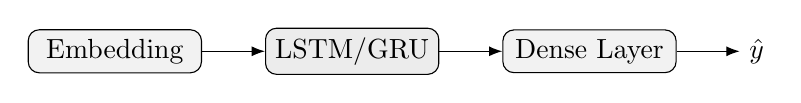
\begin{tikzpicture}[node distance=8mm, >=LaTeX]
\node[draw, rounded corners, fill=gray!10, minimum width=2.2cm] (embed) {Embedding};
\node[draw, rounded corners, right=of embed, fill=gray!15, minimum width=2.2cm] (rnn) {LSTM/GRU};
\node[draw, rounded corners, right=of rnn, fill=gray!10, minimum width=2.2cm] (fc) {Dense Layer};
\node[right=of fc] (out) {$\hat{y}$};

\draw[->] (embed) -- (rnn);
\draw[->] (rnn) -- (fc);
\draw[->] (fc) -- (out);
\end{tikzpicture}
\caption{Neural network architecture for LSTM and GRU models.}
\label{fig:rnn_architecture}
\end{figure}

\subsection{Transformer Attempt}
We attempted to fine-tune a tiny transformer using the Apple M3 Pro GPU through PyTorch’s Metal backend.  
Training repeatedly failed due to:
\begin{quote}
\small
\texttt{Insufficient Memory (kIOGPUCommandBufferCallbackErrorOutOfMemory)}
\end{quote}

Partial runs achieved accuracies above 0.80 before crashing, suggesting strong potential if trained on a device with larger GPU memory.

% --------------------------------------------------------
% 5. EXPERIMENTAL SETUP
% --------------------------------------------------------
\section{Experimental Setup}

All models are trained on the same train/test split and evaluated solely on the validation split.  
This ensures consistent and transparent comparison across architectures.

\subsection{Hardware and Software}
Experiments were conducted on:
\begin{itemize}
    \item Apple M3 Pro, 36 GB unified memory
    \item macOS Sonoma
    \item Python 3.12, PyTorch with MPS acceleration
\end{itemize}

\subsection{Hyperparameters}
For TF--IDF models:
\begin{itemize}
    \item max features: 20,000  
    \item n-grams: (1,2)
\end{itemize}

For RNNs:
\begin{itemize}
    \item embedding size: 128  
    \item hidden size: 128  
    \item dropout: 0.3  
    \item optimizer: Adam  
    \item epochs: determined by early stopping  
\end{itemize}

\subsection{Evaluation Metrics}
Due to class imbalance and the importance of minority categories (e.g., Suicidal), macro-F1 is the primary metric. Accuracy is also reported.

% --------------------------------------------------------
% 4.5 TRAINING
% --------------------------------------------------------
\section{Training}

All models were trained under a unified experimental protocol to ensure fairness, transparency, and reproducibility. 
Each model accessed the same training and test splits during optimization, while the validation split was 
reserved exclusively for final comparison across models. This section outlines the training strategies employed for 
the baseline, classical linear, and recurrent neural architectures. In addition, the full training dynamics of the 
LSTM and GRU models are visualized through learning-curve plots.

% --------------------------------------------------------
% 4.5.1 Baseline and Classical Models
% --------------------------------------------------------
\subsection{Baseline and Classical Models}

\paragraph{Majority Baseline.}
The baseline classifier required no gradient-based training. Its output was fixed to the most frequent category 
(“Normal”), establishing a minimal performance threshold.

\paragraph{TF–IDF Linear Models.}
Both Logistic Regression and Linear SVM were trained on TF–IDF features derived from unigrams and bigrams.  
Training involved optimizing the hinge loss (SVM) or cross-entropy (Logistic Regression) using the training split.  
Hyperparameters were determined through grid search on the internal test split, after which models were frozen 
and evaluated on the validation set for ranking.

% --------------------------------------------------------
% 4.5.2 Recurrent Neural Networks
% --------------------------------------------------------
\subsection{Recurrent Neural Networks}

Both RNN architectures (LSTM and GRU) were trained for 32 epochs using the Adam optimizer, batch size 64, 
embedding dimension 128, and hidden size 128. Training used early-stopping criteria monitored via validation macro-F1, 
but full 32-epoch logs are retained for scientific reporting.  
Figures~\ref{fig:lstm_curve} and~\ref{fig:gru_curve} show the complete learning curves, plotting both validation 
accuracy and macro-F1 across epochs.

% -----------------------------
% LSTM Learning Curve
% -----------------------------
\begin{figure}[h!]
\centering
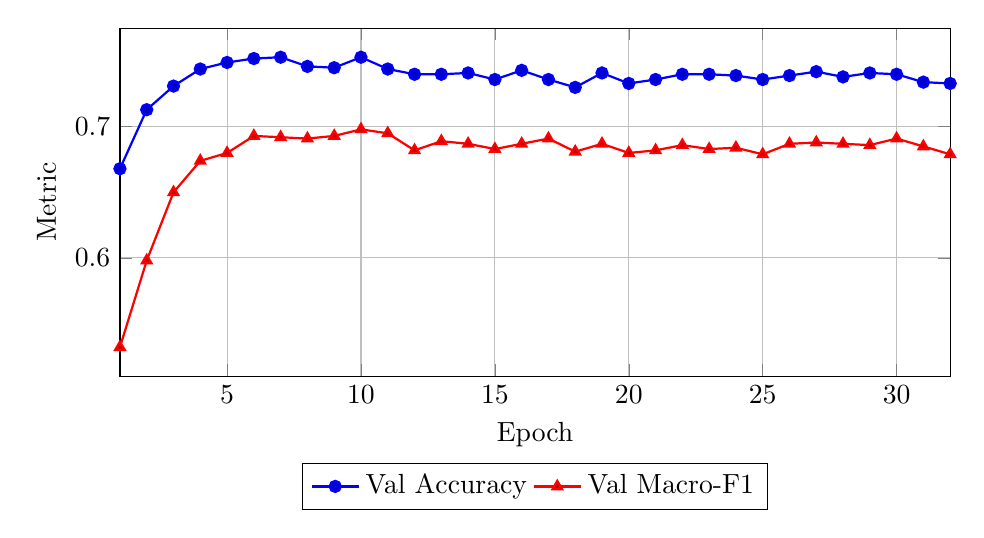
\begin{tikzpicture}
\begin{axis}[
    width=\linewidth,
    height=6cm,
    xlabel={Epoch},
    ylabel={Metric},
    xmin=1, xmax=32,
    legend style={at={(0.5,-0.25)},anchor=north,legend columns=-1},
    grid=both
]
% LSTM Accuracy
\addplot+[mark=*, thick] coordinates {
(1,0.668)(2,0.713)(3,0.731)(4,0.744)(5,0.749)(6,0.752)(7,0.753)
(8,0.746)(9,0.745)(10,0.753)(11,0.744)(12,0.740)(13,0.740)
(14,0.741)(15,0.736)(16,0.743)(17,0.736)(18,0.730)(19,0.741)
(20,0.733)(21,0.736)(22,0.740)(23,0.740)(24,0.739)
(25,0.736)(26,0.739)(27,0.742)(28,0.738)(29,0.741)
(30,0.740)(31,0.734)(32,0.733)
};
\addlegendentry{Val Accuracy}

% LSTM Macro-F1
\addplot+[mark=triangle*, thick] coordinates {
(1,0.532)(2,0.598)(3,0.650)(4,0.674)(5,0.680)(6,0.693)(7,0.692)
(8,0.691)(9,0.693)(10,0.698)(11,0.695)(12,0.682)(13,0.689)
(14,0.687)(15,0.683)(16,0.687)(17,0.691)(18,0.681)(19,0.687)
(20,0.680)(21,0.682)(22,0.686)(23,0.683)(24,0.684)
(25,0.679)(26,0.687)(27,0.688)(28,0.687)(29,0.686)
(30,0.691)(31,0.685)(32,0.679)
};
\addlegendentry{Val Macro-F1}
\end{axis}
\end{tikzpicture}
\caption{LSTM learning curves over 32 epochs.}
\label{fig:lstm_curve}
\end{figure}

% -----------------------------
% GRU Learning Curve
% -----------------------------
\begin{figure}[h!]
\centering
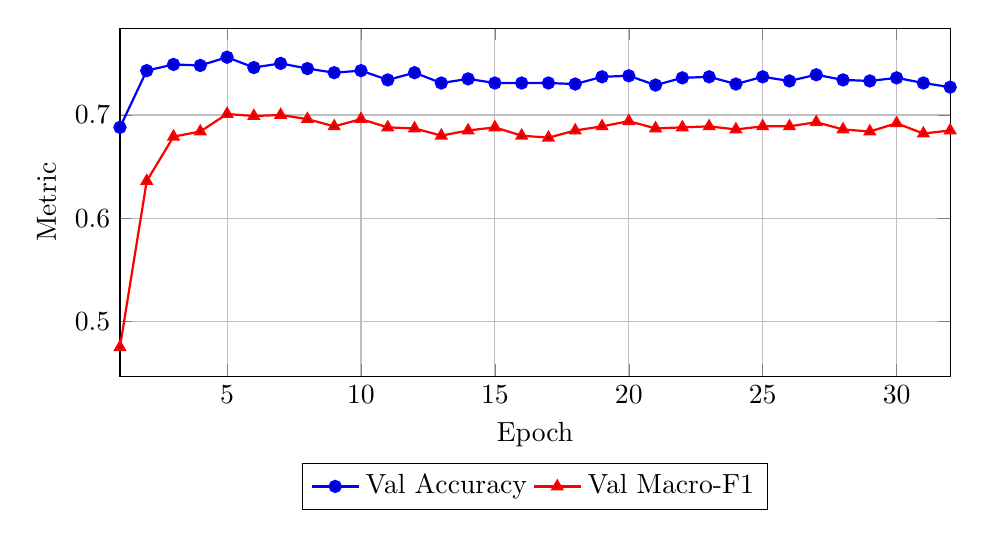
\begin{tikzpicture}
\begin{axis}[
    width=\linewidth,
    height=6cm,
    xlabel={Epoch},
    ylabel={Metric},
    xmin=1, xmax=32,
    legend style={at={(0.5,-0.25)},anchor=north,legend columns=-1},
    grid=both
]
% GRU Accuracy
\addplot+[mark=*, thick] coordinates {
(1,0.688)(2,0.743)(3,0.749)(4,0.748)(5,0.756)(6,0.746)(7,0.750)
(8,0.745)(9,0.741)(10,0.743)(11,0.734)(12,0.741)(13,0.731)
(14,0.735)(15,0.731)(16,0.731)(17,0.731)(18,0.730)(19,0.737)
(20,0.738)(21,0.729)(22,0.736)(23,0.737)(24,0.730)
(25,0.737)(26,0.733)(27,0.739)(28,0.734)(29,0.733)
(30,0.736)(31,0.731)(32,0.727)
};
\addlegendentry{Val Accuracy}

% GRU Macro-F1
\addplot+[mark=triangle*, thick] coordinates {
(1,0.475)(2,0.636)(3,0.679)(4,0.684)(5,0.701)(6,0.699)
(7,0.700)(8,0.696)(9,0.689)(10,0.696)(11,0.688)(12,0.687)
(13,0.680)(14,0.685)(15,0.688)(16,0.680)(17,0.678)(18,0.685)
(19,0.689)(20,0.694)(21,0.687)(22,0.688)(23,0.689)
(24,0.686)(25,0.689)(26,0.689)(27,0.693)(28,0.686)
(29,0.684)(30,0.692)(31,0.682)(32,0.685)
};
\addlegendentry{Val Macro-F1}
\end{axis}
\end{tikzpicture}
\caption{GRU learning curves over 32 epochs.}
\label{fig:gru_curve}
\end{figure}


% --------------------------------------------------------
% 6. RESULTS
% --------------------------------------------------------
\section{Results}

\begin{table}[h]
\centering
\caption{Model Performance on Validation Set}
\begin{tabular}{lccc}
\toprule
\textbf{Model} & \textbf{Acc} & \textbf{F1 (macro)} & \textbf{Rank} \\
\midrule
TF--IDF SVM & 0.780 & 0.749 & 1 \\
TF--IDF Logistic Reg. & 0.780 & 0.725 & 2 \\
GRU & 0.741 & 0.696 & 3 \\
LSTM & 0.744 & 0.696 & 4 \\
Majority baseline & 0.310 & 0.068 & 5 \\
Tiny Transformer* & --- & --- & --- \\
\bottomrule
\end{tabular}
\end{table}

TF--IDF models clearly outperform recurrent networks, supporting the notion that classical sparse methods remain competitive for short-text classification.

% --------------------------------------------------------
% 7. ERROR ANALYSIS
% --------------------------------------------------------
\section{Error Analysis}

Misclassifications reveal recurring patterns:
\begin{itemize}
    \item \textit{Stress} and \textit{Anxiety} often overlap semantically.
    \item \textit{Depression} dominates the dataset, leading some models to overpredict it.
    \item Rare categories (e.g., Personality Disorder) suffer from limited examples.
\end{itemize}

RNN errors commonly occur in short, ambiguous statements lacking context.

% --------------------------------------------------------
% 8. DISCUSSION
% --------------------------------------------------------
\section{Discussion}

The superior performance of TF--IDF linear models can be attributed to the dataset’s short statements and limited contextual complexity. RNNs require larger corpora to exploit sequential patterns effectively, whereas sparse n-gram features excel at capturing concise lexical cues.

The transformer model, although not fully trainable on the available hardware, showed promising results in partial runs. This aligns with the broader literature where transformers consistently outperform classical and recurrent models when trained under optimal conditions.

Ethically, automated mental-health screening must avoid overconfidence: false positives could cause unnecessary alarm, while false negatives carry significant risk. Models should support, not replace, human judgment.

% --------------------------------------------------------
% 9. CONCLUSION
% --------------------------------------------------------
\section{Conclusion}

This project provides a structured benchmark of NLP models for mental-health text classification. TF--IDF models achieved the best performance on this dataset, while RNNs performed moderately well. Preliminary transformer evidence suggests potential for superior accuracy if computational constraints are removed.

Future work includes:
\begin{itemize}
    \item full transformer fine-tuning on GPU/TPU hardware,
    \item contextual embeddings,
    \item larger datasets with more balanced class distributions,
    \item human-in-the-loop review systems.
\end{itemize}

\bibliographystyle{IEEEtran}
\begin{thebibliography}{1}

\bibitem{who2022}
World Health Organization, ``World Mental Health Report,'' 2022.

\bibitem{joachims1998}
T. Joachims, ``Text Categorization with Support Vector Machines,'' 1998.

\bibitem{hochreiter1997lstm}
S. Hochreiter and J. Schmidhuber, ``Long Short-Term Memory,'' 1997.

\bibitem{devlin2018}
J. Devlin et al., ``BERT: Pre-training of Deep Bidirectional Transformers for Language Understanding,'' 2018.

\bibitem{tausczik2010}
Y. Tausczik and J. Pennebaker, ``The Psychological Meaning of Words: LIWC and Computerized Text Analysis,'' 2010.

\end{thebibliography}

\end{document}